\section{Variable Refrigerant Flow Heat Pumps }\label{variable-refrigerant-flow-heat-pumps}

A Variable Refrigerant Flow (VRF, or Variable Refrigerant Volume) system is an air-conditioning system that varies the refrigerant flow rate using variable speed compressor(s) in the outdoor unit, and the electronic expansion valves (EEVs) located in each indoor unit. The system meets the space cooling or heating load requirements by maintaining the zone air temperature at the setpoint. The ability to control the refrigerant mass flow rate according to the cooling and/or heating load enables the use of as many as 60 or more indoor units with differing capacities in conjunction with one single outdoor unit. This unlocks the possibility of having individualized comfort control, simultaneous heating and cooling in different zones, and heat recovery from one zone to another. It may also lead to more efficient operations during part-load conditions.

There are two common types of VRF systems.

\begin{itemize}
\item
  Heat Pump (HP) type: the most general type that can be used for either cooling or heating, but not simultaneously.
\item
  Heat Recovery (HR) type: can deliver simultaneous heating and cooling to different zones by transferring heat between the cooling and heating indoor units. This generally occurs in the winter season in medium-sized to large-sized commercial buildings with a substantial core such as computer rooms.
\end{itemize}

There are two alternative VRF models availabe in EnergyPlus to simulate the energy performance of Variable Refrigerant Flow (VRF, or Variable Refrigerant Volume) air-conditioning systems:

\begin{enumerate}
\def\labelenumi{\arabic{enumi}.}
\item
  \textbf{System Curve based Model (VRF-SysCurve)}. In this model, a number of system level curves are used to describe the VRF system performance. It corresponds to the \emph{AirConditioner:VariableRefrigerantFlow} object.
\item
  \textbf{Physics based Model (VRF-FluidTCtrl)}. This model is able to consider the dynamics of more operational parameters and is applicable for fluid temperature control. This model corresponds to the \emph{AirConditioner:VariableRefrigerantFlow:FluidTemperatureControl} object.
\end{enumerate}

\subsection{Variable Refrigerant Flow Heat Pump Model (System Curve Based Model)}\label{variable-refrigerant-flow-heat-pump-model-system-curve-based-model}

\subsubsection{Overview}\label{overview-028}

This section describes the System Curve based VRF Model (VRF-SysCurve), which can address both the heat pump and heat recovery operating modes and support air-, evaporatively-, or water-cooled condenser equipment ( throughout this section, the term ``condenser'' refers to the outdoor unit where the compressor is located. )

The figure below schematically depicts the AirConditioner:VariableRefrigerantFlow (VRF AC) system. The outdoor unit is connected directly to the zone terminal units using a zone terminal unit list (ref: ZoneTerminalUnitList). The VRF AC system conditions multiple zones and is controlled by thermostats located in each zone. Zone terminal units operate to meet the zone sensible cooling or sensible heating requirements as determined by the zone thermostat schedule.

When the heat pump does not operate to reclaim waste heat, the VRF AC system can only operate in either cooling \emph{or} heating mode. Based on the master thermostat priority control selection, the operating mode is determined by polling the appropriate zone(s) served by the VRF HP system. When the system is operating in cooling mode, the cooling coils will be enabled only in the terminal units where zone cooling is required. When the system is operating in heating mode, the heating coils will be enabled only in the terminal units where zone heating is required. Supply air fans will continue to operate if the zone terminal unit's fan operating mode is set to continuous fan.

When the heat pump does operate to reclaim waste heat, the VRF AC system can simultaneously cool and heat multiple zones. The heat pump will select an operating mode according to the dominant load as reported by the zone thermostat(s). The calculation of the dominant load is based on the master thermostat priority control selection and may either be based on individual zone loads, the number of zones requiring cooling or heating, the master thermostat zone load, or an operating mode schedule. The heat pump will operate in cooling mode, and provide waste heat to zones with a heating load, when the dominant load among all zone terminal units is cooling. The heat pump will operate in heating mode, and absorb heat from zones with a cooling load, when the dominant load among all zone terminal units is heating.

The figure below shows the VRF AC terminal units with draw through fan placement. Blow through fan placement can also be modeled by connecting the supply air fan inlet node to the outside air mixer's mixed air node if an outdoor air mixer is used or to the zone terminal unit inlet node if an outdoor air mixer is not used. The variable refrigerant flow heat pump coordinates the operation of these components and is modeled as a type of zone equipment where the \emph{zone terminal units} are specified in a zone equipment list (Ref. ZoneHVAC: EquipmentList and ZoneHVAC:EquipmentConnections). The AirConditioner: VariableRefrigerantFlow object \emph{is not} specified in an air primary loop or a zone equipment list object.

\begin{figure}[hbtp] % fig 242
\centering
\includegraphics[width=0.9\textwidth, height=0.9\textheight, keepaspectratio=true]{media/image5315.png}
\caption{Variable Refrigerant Flow Heat Pump (draw through fan placement) \protect \label{fig:variable-refrigerant-flow-heat-pump-draw}}
\end{figure}

\begin{figure}[hbtp] % fig 243
\centering
\includegraphics[width=0.9\textwidth, height=0.9\textheight, keepaspectratio=true]{media/image5316.png}
\caption{Energyplus object connections for VRF-SysCurve model \protect \label{fig:energyplus-object-connections-for-vrf}}
\end{figure}

The terminal unit is able to model supply air fan operation in two modes: cycling fan -- cycling coil (i.e., AUTO fan) and continuous fan -- cycling coil (i.e., fan ON). Fan:Simple:OnOff must be used to model AUTO fan, while Fan:Simple:OnOff or Fan:Simple:ConstVolume can be used to model fan ON.

Output variables reported by the VRF AC object include the heat pump's operating capacity (cooling or heating), electric consumption, operating COP, defrost electric consumption, part-load ratio (ratio of actual capacity to available capacity), runtime fraction (when cycling), cycling ratio (actual compressor cycling rate), crankcase heater power, and other report variables associated with an evaporative condenser. Report variables are also available to indicate the maximum available terminal unit cooling or heating capacity (i.e., when the condensers available capacity is insufficient to supply the capacity requested by all terminal units). Reporting of other variables of interest for the VRF AC (fan electric power, DX coil cooling rate, DX coil heating rate, terminal unit total cooling rate, etc.) is done by the individual system components (e.g., fan, DX cooling coil, DX heating coil, and zone terminal unit). For convenience, the total cooling and heating coil capacities (i.e., the coil loads) is also reported.

\subsubsection{Model Description}\label{model-description-015}

As described previously, the VRF AC system conditions multiple zones and is controlled by one or more zone thermostats (ZoneControl:Thermostatic). Each simulation time step, EnergyPlus performs a zone air heat balance to determine if cooling or heating is required to meet each zone's thermostat set point. When heat pump mode is selected (i.e., heat recovery is not selected), an operating mode is chosen based on the master thermostat priority control and all terminal units are operated in that specific mode. When heat recovery mode is selected, the dominant load is determined based on the master thermostat priority control and the outdoor unit operates in this mode. The indoor terminal units operate in either cooling or heating mode based on the individual coil loads The heat pump condenser is then modeled to determine any impact the condensing unit might have on the zone terminal units (i.e., capacity limitations due to oversized terminal units, operating limitations due to allowable operating temperature range, impacts of defrost operation, changes in performance when heat recovery mode is active, etc.). The following sections describe the performance calculations for cooling and heating.

\subsubsection{Cooling Operation}\label{cooling-operation-000}

The operating capacity of the heat pump is calculated based on the user defined input for the heat pump's rated cooling capacity, the ratio of indoor terminal unit capacity to outdoor unit capacity (combination ratio), the actual operating conditions, and whether or not the system's heat recovery mode is active. Performance correction factors are used to correct for off-design performance as follows:

\subsubsection{Cooling Combination Ratio Correction Factor}\label{cooling-combination-ratio-correction-factor}

The cooling combination ratio correction factor is defined as the total terminal unit rated cooling capacity divided by the heat pump's rated cooling capacity. The combination ratio is important when multiple terminal units (or DX coils) are attached to a single variable-speed condensing unit. If the combination ratio is less than 1, the condenser's rated capacity is assumed to be able to meet the indoor terminal unit's demand request. However, if the combination ratio is determined to be greater than 1, the maximum cooling capacity available from the heat pump's condenser may be higher than the user specified rated cooling capacity. The combination ratio capacity correction factor is based on a linear, quadratic or cubic curve and provides a multiplier \textgreater{} 1 to correct for combination ratio's greater than 1. For example, a combination ratio of 1.3 (130\%) may result in a combination ratio capacity correction factor of 1.06 (outdoor condenser can actually provide 106\% of rated capacity) . The cooling combination ratio correction factor is applied to cooling performance calculations. If the cooling combination ratio correction curve name is not specified by the user, the cooling combination ratio correction factor (CR \(_{cooling,\, correction}\)) in the following equation is assumed to be equal to 1.

\begin{equation}
  CR_{cooling,rated} = \frac{\sum \limits_1^n \dot{Q}_{coil(i),cooling,rated}}{\dot{Q}_{cooling,total,rated}}
\end{equation}

\begin{equation}
C{R_{\,cooling\,,\,correction}} = a + b\left( {C{R_{cooling\,,\,rated}}} \right) + c{\left( {C{R_{cooling\,,\,rated}}} \right)^2} + d{\left( {C{R_{cooling\,,\,rated}}} \right)^3}
\end{equation}

\begin{equation}
C{R_{\,cooling\,,\,correction}} = MAX\left( {1.0\,\,,\,\,C{R_{\,cooling\,,\,correction}}} \right)
\end{equation}

where

\({\mathop Q\limits^ \bullet_{coil(i)\,,\,cooling\,,\,rated}}\) ~ = rated total (sensible + latent) cooling capacity in zone \emph{i} (W)

\({\mathop Q\limits^ \bullet_{cooling,\,total\,,\,rated}}\) ~~ = rated total cooling capacity of heat pump (W)

\(C{R_{\,cooling\,,\,correction}}\) ~ = Cooling Combination Ratio capacity correction factor at rated conditions (this value is reported in the eio file)

\(a - d\) ~~~~~~~ ~~~~~~~ = equation coefficients for cooling combination ratio correction factor

\(C{R_{cooling\,,\,rated}}\) ~~ ~~~ = the cooling combination ratio defined as the total indoor terminal unit's rated total cooling capacity divided by the rated total cooling capacity of the heat pump condenser.

The sum of the individual zone total cooling requirements is used to calculate the performance of the outdoor condensing unit. The operating capacities of the indoor cooling coils are calculated based on the indoor cooling coil's rated cooling capacity and the actual operating conditions. The operating capacity of the heat pump condenser is calculated in a similar fashion using a load-weighted average indoor wet-bulb temperature of all operating cooling coils.

\subsubsection{Cooling Capacity Ratio Modifier Function of Low Temperature}\label{cooling-capacity-ratio-modifier-function-of-low-temperature}

The heat pump's cooling capacity correction factor (function of temperature) is determined by averaging the zone cooling coil inlet air wet-bulb temperature for all operating cooling coils. A load-weighted average inlet air wet-bulb temperature is used in the calculations. The weighted average cooling coil inlet air wet-bulb temperature and the outdoor condenser entering air dry-bulb temperature are then used to calculate the temperature correction factor in cooling mode for the heat pump condenser. The actual zone air wet-bulb temperature is used to calculate the operating capacity of the individual zone cooling coils.

\begin{equation}
{\mathop Q\limits^ \bullet_{zone,\,total}} = \sum\limits_1^i {{{\mathop Q\limits^ \bullet  }_{zone(i)}}}
\end{equation}

\begin{equation}
  T_{wb,avg} = \sum\limits_1^i {\PB{T_{wb,i}}} \PB{\dot{Q}_{zone(i)}}{\dot{Q}_{zone,total}}
\end{equation}

The operating capacity of the heat pump is calculated using a bi-quadratic equation using a load-weighted average indoor wet-bulb temperature and outdoor dry-bulb temperature as the independent variables.

\begin{equation}
CAPF{T_{HP,cooling}} = a + b\left( {{T_{wb,avg}}} \right) + c{\left( {{T_{wb,avg}}} \right)^2} + d\left( {{T_c}} \right) + e{\left( {{T_c}} \right)^2} + f\left( {{T_{wb,avg}}} \right)\left( {{T_c}} \right)
\end{equation}

The operating capacity of the terminal unit's DX cooling coil is calculated using either a linear, quadratic, or cubic curve. If more information is available to more accurately model the DX cooling coil, a bi-quadratic curve may be used (i.e., if the performance of the DX cooling coil is also a function of outdoor dry-bulb temperature).

\begin{equation}
CAPF{T_{coil,\,cooling}} = a + b\left( {{T_{wb,i}}} \right) + c{\left( {{T_{wb,i}}} \right)^2} + d{\left( {{T_{wb,i}}} \right)^3}
\end{equation}

~- or -

\begin{equation}
CAPF{T_{coil,cooling}} = a + b\left( {{T_{wb,i}}} \right) + c{\left( {{T_{wb,i}}} \right)^2} + d\left( {{T_c}} \right) + e{\left( {{T_c}} \right)^2} + f\left( {{T_{wb,i}}} \right)\left( {{T_c}} \right)
\end{equation}

where

\({T_{wb,i}}\) ~ = wet-bulb temperature of the air entering the cooling coil in zone \emph{i} (°C)

\({T_{wb,avg}}\) = load-weighted average wet-bulb temperature of the air entering all operating cooling coils (°C)

\({\mathop Q\limits^ \bullet_{zone(i)}}\) ~ = total (sensible + latent) cooling load in zone \emph{i} (W)

\({\mathop Q\limits^ \bullet_{zone,\,total}}\) ~ = total (sensible + latent) cooling load in all zones (W)

\(CAPF{T_{\,HP,cooling}}\) ~ = heat pump Cooling Capacity Ratio Modifier (function of temperature)

\(CAPF{T_{\,coil,cooling}}\) ~ = zone coil Cooling Capacity Ratio Modifier (function of temperature)

\(a - f\) ~ = equation coefficients for Cooling Capacity Ratio Modifier

\({T_c}\) ~~~ = temperature of the air entering an air-cooled or evaporatively-cooled condenser (°C)

\subsubsection{Using multiple curves to define Cooling Capacity Ratio Modifier}\label{using-multiple-curves-to-define-cooling-capacity-ratio-modifier}

The cooling capacity ratio modifier determines the change in total (sensible + latent) capacity with respect to the heat pump rated cooling capacity. This modifier corrects for off-design performance and provides the operating total (sensible + latent) cooling capacity for the heat pump condenser. The performance data for VRF AC systems may be specified using a single curve object, however, if the performance data does not reflect a smooth change in performance as outdoor conditions vary, the overall performance of the system may be described using two cooling capacity ratio modifier curves (i.e., a separate curve at low and high outdoor temperatures) and a boundary curve (i.e., the curve defining the separation at specific outdoor temperatures).

\subsubsection{Application of Dual Performance Curves}\label{application-of-dual-performance-curves}

Two additional inputs are available to more accurately model the cooling performance of a VRF AC system. The first additional input is a boundary curve which is used to distinguish differences in performance at ``low'' and ``high'' outdoor temperature regions and the second input is a cooling capacity performance curve for the ``high'' outdoor temperature region. The boundary curve is a linear, quadratic or cubic curve defining the outdoor temperature as a function of average indoor wet-bulb temperature. The cooling capacity ratio function of high temperature curve is a biquadratic curve using average indoor wet-bulb temperature and outdoor dry-bulb temperature as the two independent variables. These additional curves are used to define the performance over two separate performance regions as shown in Figure 244. The red circles in the figure identify the points at which the performance changes abruptly (i.e., slopes or shapes are significantly different) and are used to create the boundary curve. The performance on either side of the boundary curve can be a smooth curve changing with outdoor condition or a flat plateau where system controls maintain a constant operating condition. This type of performance cannot be accurately simulated using a single performance curve object. For this reason, dual capacity performance curves may be used.

Note: If the cooling performance can be described using a single performance curve object, the boundary and high temperature performance curve objects are not required.

Manufacturers may also provide this information in a tabular format. In this case the data should first be graphically displayed to identify any non-linearities and to also identify where an abrupt change in performance occurs so that a boundary curve can be created.

The cooling capacity ratio boundary curve object is used to differentiate between dual cooling capacity ratio performance curves. This curve defines the outdoor temperature below which the cooling capacity ratio function of low temperature curve object is used, otherwise, the cooling capacity ratio function of high temperature curve object is used.

\begin{equation}
{T_{OA,DB}} = a + b\left( {{T_{I,WB}}} \right) + c{\left( {{T_{I,WB}}} \right)^2} + d{\left( {{T_{I,WB}}} \right)^3}
\end{equation}

where

T\(_{OA,DB}\) = Outside air dry-bulb temperature (C)

a-d = coefficients for cooling capacity ratio boundary curve object

T\(_{I,WB}\) = Weighted average indoor wet-bulb temperature (C)

For the performance data shown below, the boundary curve would be created by identifying the outdoor dry-bulb temperature at which the performance changed abruptly for each of the indoor wet-bulb temperature curves shown in the figure. The following example shows the data interpreted from the figure used to regress the cooling capacity ratio boundary curve coefficients. For this example, the regression coefficients were found to be: A1 = 29.87396, B1 = -0.6928, C1 = 0.01928, D1 = -0.000532

\begin{figure}[hbtp] % table 73
\centering
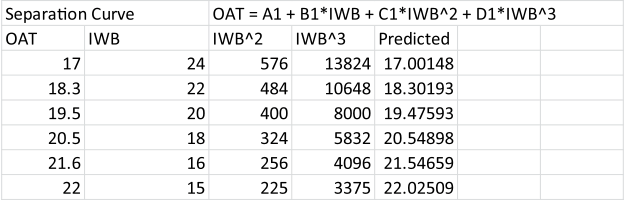
\includegraphics[width=0.9\textwidth, height=0.9\textheight, keepaspectratio=true]{media/image5339.png}
\caption{Performance Data for Variable Refrigerant Flow Air Conditioner Model \label{fig:performance-data-for-variable-refrigerant-flow-air-conditioner-model}}
\end{figure}


\begin{enumerate}
\def\labelenumi{\alph{enumi}.}
\setcounter{enumi}{1}
\tightlist
\item
  Find the \(rps\) range that covers the required evaporative capacity \(Q_{rps,modify}\) .
\end{enumerate}

\begin{equation}
Q_{rps,modify} = C_{cap,operation}\times(\sum{Q_{in,total}}+Q_{pipe})
\end{equation}

\begin{equation}
C_{cap,operation} = C_{cap,density}\times{C_{cap,enthalpy}}
\end{equation}

\begin{equation}
C_{cap,density} = \rho_{test}/\rho_{real}
\end{equation}

\begin{equation}
C_{cap,enthalpy} = \frac{h_{Evapout,test}-h_{Evapin,test}}{h_{Compin,real}-h_{Evapin,real}}
\end{equation}

\begin{equation}
h_{Compin,real} = h_{Hexout,real}+Q_{pipe}/G_{tot}
\end{equation}

Where

\(C_{cap,operation}\) evaporative capacity correction factor, describing the operational difference between test cases and real cases (i.e., \(SH\) and \(SC\) )

\(C_{cap,density}\) evaporative capacity correction factor, describing the variations of refrigerant density at test conditions and real operational conditions

\(C_{cap,enthalpy}\) evaporative capacity correction factor, describing the variations of refrigerant enthalpy at test conditions and real operational conditions

\(G_{tot}\) refrigerant flow rate in the main loop (kg/s)

\(h_{Evapin,real}\) enthalpy of refrigerant entering the evaporators (IU) at real conditions {[}kJ/kg{]}

\(h_{Evapout,real}\) average enthalpy of refrigerant leaving the evaporators (IU) at real conditions {[}kJ/kg{]}

\(h_{Evapin,test}\) enthalpy of refrigerant entering the evaporator at test conditions (It corresponds to \(SC\) at test condition(e.g., 5 °C) and Tc) (kJ/kg)

\(h_{Evapout,test}\) enthalpy of refrigerant leaving the evaporator at test conditions (It corresponds to \(SH\) at test condition(e.g., 8 °C) and Te) (kJ/kg)

\(h_{Compin}\) enthalpy of refrigerant entering the compressor (kJ/kg)

\(Q_{pipe}\) heat loss through the pipe (W)

For example, if the required capacity is 8 kW, the \(rps\) range is 30 to 36.

\begin{enumerate}
\def\labelenumi{\alph{enumi}.}
\setcounter{enumi}{2}
\item
  Calculate the \(rps\) that meets the required capacity by interpolation. In the above example, the resulting \(rps\) is 34.5 \(rps\) .
\item
  If the calculated \(rps\) is lower than the minimum \(rps\) (e.g.~18\(rps\) ), go to Step 2c.5, otherwise skip Step 2c.5 and directly go to Step 2c. 6.
\end{enumerate}

\paragraph{Step 2c.5: Modify evaporating temperature to further reduce outdoor unit capacity}\label{step-2c.5-modify-evaporating-temperature-to-further-reduce-outdoor-unit-capacity}

If the calculated \(rps\) is lower than the minimum \(rps\) (e.g.~18\(rps\) ), it means that the zone cooling load is even lower than the system evaporative capacity corresponding to the minimum compressor speed. In this situation, the evaporating temperature \(T_e\) as well as the superheating degree \(SH\) is modified to further reduce the outdoor unit capacity. More specifically:

\begin{enumerate}
\def\labelenumi{\alph{enumi}.}
\item
  Set \(rps\) at its minimum value (e.g., 18 \(rps\) ).
\item
  Update \({T_e}'\) to meet the required evaporative capacity, using equations described in Step 2c.4a.
\item
  Update \(T_e\) to meet the updated \({T_e}'\) . Note that due to the \(T_e\) updates, the refrigerant state and flow rate are changed and thus the piping loss analysis should also be repeated (Step 2c.1). So is the calculation of \(C_{cap,operation}\) (Step 2c.2-2c.3).
\item
  \(SH\) can be updated based on the updated \(T_e\) , using the equations shown in Step 1.2.
\end{enumerate}

\paragraph{Step 2c.6: Calculate the compressor power}\label{step-2c.6-calculate-the-compressor-power}

\begin{enumerate}
\def\labelenumi{(\arabic{enumi})}
\tightlist
\item
  Calculate the compressor power by the following procedures. 
\end{enumerate}

\begin{enumerate}
\def\labelenumi{\alph{enumi}.}
\tightlist
\item
  Calculate the compressor power at a variety of loading index using the following equation. The resulting table (Table 2) from the same example used above is shown below.
\end{enumerate}

\[M_{comp} = c_1+c_2T_c+c_3{T_e}'+c_4T_c^2+c_5T_c{T_e}'+c_6{T_e}'^2\] \[N_{comp,rps} = M_{comp} \times N_{comp,ref}\]

Where

\(c_1\) ,\ldots{},\(c_6\) empirical coefficients corresponding to \(rps\)

\({T_e}'\) suction saturated temperature at the compressor inlet (°C)

\(T_c\) effective condensing temperature (°C)

\(M_{comp}\) multiplier for the compressor power calculation (--)

\(N_{comp,ref}\) rated compressor power (W)

\(N_{comp,rps}\) compressor power corresponding to \(rps\) (W)

Table 2 -- Outdoor unit compressor power at different Loading Index



\begin{enumerate}
\def\labelenumi{\alph{enumi}.}
\setcounter{enumi}{1}
\tightlist
\item
  According to the \(rps\) range determined, calculate the compressor power \(N_{comp}\) by interpolation. In the above example, the compressor power is 1.155 kW. 
\end{enumerate}

\begin{enumerate}
\def\labelenumi{(\arabic{enumi})}
\setcounter{enumi}{1}
\tightlist
\item
  Compare the calculated \(N_{comp}\) above with the initialized \({N_{comp}}'\) in Step 2c.2:
\end{enumerate}

\begin{itemize}
\item
  If \({N_{comp}}'-N_{comp}>\delta\) then go to Step 2c.2 for a new round of iteration.
\item
  Else, end the iteration and go to Step 2c.7.
\end{itemize}

\paragraph{Step 2c.7: Total power consumption of the outdoor unit}\label{step-2c.7-total-power-consumption-of-the-outdoor-unit}

Calculate the total electric power consumption by the outdoor unit:

\begin{equation}
N_{out} = N_{fan}+N_{comp}/e_{inv}
\end{equation}

Where

\(e_{inv}\) efficiency of the inverter of compressor

\(N_{fan}\) electric power consumption by the outdoor fan (W)

\(N_{out}\) total electric power consumption by the outdoor unit (W)

\subsubsection{\texorpdfstring{\emph{Modeling of the outdoor unit (O/U) - Heating Mode}}{Modeling of the outdoor unit (O/U) - Heating Mode}}\label{modeling-of-the-outdoor-unit-ou---heating-mode}

\paragraph{Step 2h.1: Piping loss calculation in the heating mode}\label{step-2h.1-piping-loss-calculation-in-the-heating-mode}

Similarly to that in the cooling mode, the piping loss analysis in the heating mode needs to address the coupling effect between the piping loss and system operations. However, due to the control strategy difference between the two modes, the piping loss algorithm in the heating mode requires different calculation steps and more numerical iterations, as shown below.

Calculate the refrigerant flow rate for each indoor unit using assumed \(h_{Hexin}\) :

\begin{equation}
G_i = Q_i/(h_{Hexin}-h_{Hexout,i})
\end{equation}

Where

\(G_i\) refrigerant flow rate for the i\(^{th}\) indoor unit (kg/s)

\(Q_i\) total heating load of the i\(^{th}\) zone (W)

\(h_{Hexin}\) enthalpy of the refrigerant entering the indoor unit (kJ/kg)

\(h_{Hexout,i}\) enthalpy of the refrigerant leaving a specific indoor unit (kJ/kg)

\(h_{Hexout,i}\) is a function of \(P_c\) , \(T_c\) , and \(SC_i\) . It can be calculated using refrigerant thermodynamic property equations \(f_{g_h}(P_c,T_c-SC_i)\) .

The refrigerant flow rate in the main loop can be obtained by summing up the flow rate in each indoor unit:

\begin{equation}
G_{tot} = \sum{G_i}
\end{equation}

Where

\(G_{tot}\) refrigerant flow rate in the main loop (kg/s)

Calculate the average refrigerant pressure and enthalpy within the pipes, using assumed piping pressure loss \(\Delta{P_{pipe}}\) and \(h_{Tdi}\) :

\begin{equation}
P_{ave} = P_c+\Delta{P_{pipe}}/2
\end{equation}

\begin{equation}
h_{ave} = (h_{Hexin}+h_{Tdi})/2
\end{equation}

Where

\(h_{ave}\) average refrigerant enthalpy within the main pipe (kJ/kg)

\(h_{Hexin}\) enthalpy of the refrigerant entering the indoor unit (kJ/kg)

\(h_{Tdi}\) enthalpy of the refrigerant leaving the compressor (kJ/kg)

\(P_{ave}\) average refrigerant pressure within the main pipe (Pa)

\(P_c\) condensing pressure (Pa)

\(\Delta{P_{pipe}}\) pressure drop in the main pipe (Pa)

The viscosity of the refrigerant within the pipe can be calculated given \(P_{ave}\) and \(h_{ave}\) , using the following equations:

\begin{equation}
k_{v,1} = P_{ave}/4926000
\end{equation}

\begin{equation}
k_{v,2} = h_{ave}/383.55
\end{equation}

\begin{equation}
k_{v,3} = (T_{ave}+273.15)/344.39
\end{equation}

\begin{equation}
\mu = 10^6\times(4.302\times{k_{v,1}}+0.81622\times{k_{v,1}}^2-120.98\times{k_{v,2}}+139.17\times{k_{v,2}}^2+118.76\times{k_{v,3}}+81.04\times{k_{v,3}}^2+5.7858\times{k_{v,1}}\times{k_{v,2}}-8.3817\times{k_{v,1}}\times{k_{v,3}}-218.48\times{k_{v,2}}\times{k_{v,3}}+21.58)
\end{equation}

Where

\(\mu\) viscosity of the refrigerant within the pipe (Pa-s)

\(k_{v,i}\) coefficients to calculate the refrigerant viscosity

\(h_{ave}\) average refrigerant enthalpy within the pipes (kJ/kg)

\(P_{ave}\) average refrigerant pressure within the pipes (Pa)

\(T_{ave}\) average temperature of refrigerant leaving indoor units, which corresponds to \(P_{ave}\) and \(h_{ave}\) (°C)

Given \(P_{ave}\) and \(h_{ave}\) , the following dimensionless quantities describing the refrigerant flow state can be obtained:

\begin{equation}
Re = G_{tot}/3600/(0.25\times\pi\times{D^2})\times{D}/\mu
\end{equation}

\begin{equation}
Pr = \mu\times{f_{g_Cp}(P_{ave},h_{ave})}\times{0.001}/f_{g_\lambda}(P_{ave},h_{ave})
\end{equation}

\begin{equation}
Nu = 0.023\times{Re^{0.8}\times{Pr^{0.4}}}
\end{equation}

\begin{equation}
St = Nu/Re/Pr
\end{equation}

Where

\(Re\) Reynolds number

\(Pr\) Prandtl number

\(Nu\) Nusselt number

\(St\) Stanton number

\(\mu\) viscosity of the refrigerant within the pipe (Pa-s)

\(f_{g_Cp}\) functions calculating the specific heat of superheating refrigerant

\(f_{g_\lambda}\) functions calculating the conductivity of superheating refrigerant

Then the piping pressure loss \(\Delta{P_{pipe}}\) can be obtained using the above dimensionless quantities:

\begin{equation}
\Delta{P_{pipe}} = 8\times{St}\times{Pr^{2/3}}\times{L/D}\times{f_{g_\rho}(P_{ave},h_{ave})}\times{V^2}/2-H\times{f_{g_\rho}(P_{ave},h_{ave})}\times9.80665
\end{equation}

Where

\(f_{g_\rho}\) functions calculating the density of superheating refrigerant

\(D\) main pipe diameter (m)

\(H\) height difference between the outdoor unit node and indoor unit node of the main pipe (m)

\(L\) main pipe length (m)

\(St\) Stanton number

\(Re\) Reynolds number

\(Pr\) Prandtl number

\(\Delta{P_{pipe}}\) pressure drop in the pipe (Pa)

\(V\) refrigerant flow velocity (m/s)

Compare the calculated \(\Delta{P_{pipe}}\) and the one assumed above. If the difference is higher than the assigned tolerance (5\%), a new round of iteration is performed using the calculated \(\Delta{P_{pipe}}\) .

The compressor discharge saturated temperature \(T'_c\) (i.e., saturated vapor temperature corresponding to compressor discharge pressure) can be obtained via:

\begin{equation}
T'_c = f_{s_t}(P_c+\Delta{P_{pipe}})
\end{equation}

Where

\(f_{s_t}\) functions calculating the temperature of saturated refrigerant

\(T'_c\) discharge saturated temperature at the compressor outlet (°C)

\(P_c\) condensing pressure (Pa)

\(\Delta{P_{pipe}}\) pressure drop in the pipe (Pa)

The heat loss through the pipe can be obtained via:

\begin{equation}
k_1 = Nu\times{f_{g_\lambda}(P_{ave},h_{ave})}
\end{equation}

\begin{equation}
k_2 = 2\times{\lambda_i}/Ln(1+2\times{W_i}/D)
\end{equation}

\begin{equation}
k_3 = h\times(D+2\times{W_i})
\end{equation}

\begin{equation}
Q_{pipe} = (\pi\times{L})\times(T_a-T_{Hexin})/(1/k_1+1/k_2+1/k_3)
\end{equation}

Where

\(f_{g_\lambda}\) functions calculating the conductivity of superheating refrigerant

\(Q_{pipe}\) heat loss through the pipe (W)

\(T_a\) average of outdoor air temperature and indoor temperature (°C)

\(T_{Hexin}\) average of entering indoor units (°C)

\(w_i\) pipe insulation thickness (m)

\(k_i\) coefficients for the piping loss calculation

The enthalpy of the refrigerant entering the indoor unit can be updated using the calculated \(Q_{pipe}\) :

\begin{equation}
h_{Tdi} = h_{Hexin}+Q_{pipe}/G_{tot}
\end{equation}

Where

\(h_{Hexin}\) enthalpy of the refrigerant entering the indoor unit (kJ/kg)

\(h_{Tdi}\) enthalpy of the refrigerant leaving the compressor (kJ/kg)

\(G_{tot}\) refrigerant flow rate in the main loop (kg/s)

Compare the calculated \(h_{Tdi}\) and the one assumed above. If the difference is higher than the assigned tolerance (5\%), a new round of iteration is performed using the calculated \(h_{Tdi}\) .

Note that \(Q_{pipe}\) is calculated using an assumed \(h_{Hexin}\) at the beginning of the piping loss algorithm. Its value affects the compressor operation calculations as shown in Step 2h.2\textasciitilde{}2h.6 and may change the value of evaporating temperature \(T_e\) . This leads to an updated \(h_{Hexin} = f(P_e,T_e+SH,N_{comp},G_{tot})\) . If the difference between the calculated result and the assumed value is higher than the assigned tolerance (5\%), a new round of iteration is performed using the calculated \(h_{Hexin}\) .

\paragraph{Step 2h.2: Initialize O/U operation conditions}\label{step-2h.2-initialize-ou-operation-conditions}

Similar to that in cooling mode, an iteration approach is designed to determine the energy consumption of the compressor (Step 2h. 2 to Step 2h. 6).

For the first iteration,

\begin{itemize}
\item
  Initialize outdoor unit \(SH\) with the reference value (from IDF input, e.g., 1.5°C)
\item
  Iinitialize the compressor power \(N_{comp}\) with the value calculated from the reference \(COP\) (e.g., 3.5):
\end{itemize}

\begin{equation}
N'_{comp} = \frac{\sum_iQ_{in,total,i}}{COP}
\end{equation}

Where

\(N_{comp}\) compressor power (W)

\(N'_{comp}\) assumed compressor power for the first iteration (W)

\(Q_{in,total,i}\) total heating load for zone \(i\) (W)

For the following iterations,

\begin{itemize}
\item
  Initialize \(SH\) with the calculated value in the previous iteration
\item
  Initialize the compressor power \(N_{comp}\) with the calculated value in the previous iteration
\end{itemize}

Calculate the heat rate extracted by the outdoor unit by:

\begin{equation}
Q_{out} = \sum_iQ_{in,total,i}+Q_{pipe}-N_{comp}
\end{equation}

Where

\(Q_{out}\) heat rate extracted by the outdoor unit (W)

\(Q_{pipe}\) heat loss through the pipe (W)

\paragraph{Step 2h.3: Calculate O/U effective evaporating temperature}\label{step-2h.3-calculate-ou-effective-evaporating-temperature}

\begin{enumerate}
\def\labelenumi{(\arabic{enumi})}
\tightlist
\item
  Calculate the required coil surface air temperature \({T_{fs}}'\) for the outdoor unit.
\end{enumerate}

The enthalpy of the air leaving the outdoor unit can be calculated by:

\begin{equation}
{H_{fs}}' = {H_{in}}'-Q_{out}/({G_{a,rate}}'\times{\rho_o})/(1-BF')
\end{equation}

The coil surface air temperature \({T_{fs}}'\) can be calculated from the \({H_{fs}}'\) :

\begin{equation}
if\quad{H_{fs}}'<H_{98\%,W_o}\quad{then}\quad{T_{fs}}' = f({H_{fs}}',98\%)
\end{equation}

\begin{equation}
if\quad{H_{fs}}'\ge{H_{98\%,W_o}}\quad{then}\quad{T_{fs}}' = f({H_{fs}}',W_o)
\end{equation}

Where

\(BF'\) bypass factor for the outdoor unit

\({G_{a,rate}}'\) volumetric flow rate of the air through the outdoor unit, at the rating conditions (m\(^{3}\)/s)

\({H_{fs}}'\) enthalpy of the air leaving the outdoor unit (kJ/kg)

\({H_{in}}'\) enthalpy of the air entering the outdoor unit, i.e., outdoor air (kJ/kg)

\(W_o\) humidity ratio of the outdoor air (kg/kg)

\(\rho_o\) density of the outdoor air (kg/m\(^{3}\))

\begin{enumerate}
\def\labelenumi{(\arabic{enumi})}
\setcounter{enumi}{1}
\tightlist
\item
  Calculate required evaporating temperature for the outdoor unit \(Te_{req}\) and then the effective evaporating temperature \(Te\) .
\end{enumerate}

\begin{equation}
Te_{req} = {T_{fs}}'-[{A_c}'\cdot SH^2+{B_c}'\cdot SH+{C_c}']
\end{equation}

\begin{equation}
Te = Te_{req}
\end{equation}

Where

\({A_c}'\) ,\({B_c}'\) ,\({C_c}'\) coefficients (°C)

\(SH\) superheating degrees for the outdoor unit (°C)

\(SH_{ref}\) reference superheating degrees for the outdoor unit (°C)

\(Te_{req}\) required evaporating temperature for the outdoor unit (°C)

\(Te\) effective evaporating temperature (°C)

\paragraph{Step 2h.4: Calculate required compressor Loading Index}\label{step-2h.4-calculate-required-compressor-loading-index}

Calculate the required compressor Loading Index by the following procedures.

\begin{enumerate}
\def\labelenumi{\alph{enumi}.}
\tightlist
\item
  Calculate the evaporative capacity at a variety of speeds:
\end{enumerate}

\[M_{cap} = C_{cap,system}\times(r_1+r_2{T_c}'+r_3T_e+r_4{T_c}'^2+r_5{T_c}'T_e+r_6T_e^2)\] \[Q_{rps} = C_{cap,system} \times M_{cap} \times Q_{ref}\]

Where

\(C_{cap,system}\) evaporative capacity correction factor, describing the possible system configuration difference between test bed and real system (obtained from manufacturer data)

\(r_1\) ,\ldots{},\(r_6\) empirical coefficients corresponding to \(rps\)

\(rps\) compressor speed (r/s)

\(T_e\) effective evaporating temperature (°C)

\(M_{cap}\) multiplier for the evaporative capacity calculation (--)

\({T_c}'\) discharge saturated temperature at the compressor outlet (°C)

\(Q_{rps}\) evaporative capacity corresponding to \(rps\) (W)

\(Q_{ref}\) rated evaporative capacity (W)

An example of resulting capacity for different \(rps\) (at \({T_c}'\) = 36°C and \(T_e\) = 9°C) is presented in Table 3.

Table 3-- evaporative capacity at different Loading Index



\begin{enumerate}
\def\labelenumi{\alph{enumi}.}
\setcounter{enumi}{1}
\tightlist
\item
  Find the \(rps\) range that covers the required evaporative capacity \(Q_{rps,modify}\) .
\end{enumerate}

\begin{equation}
Q_{rps,modify} = C_{cap,operation}\times(\sum{Q_{in,total}}+Q_{pipe}-N_{comp})
\end{equation}

\begin{equation}
C_{cap,operation} = C_{cap,density}\times{C_{cap,enthalpy}}
\end{equation}

\begin{equation}
C_{cap,density} = \rho_{test}/\rho_{real}
\end{equation}

\begin{equation}
C_{cap,enthalpy} = \frac{h_{Evapout,test}-h_{Condout,test}}{h_{Compin,real}-h_{Condout,real}}
\end{equation}

Where

\(C_{cap,operation}\) evaporative capacity correction factor, describing the operational difference between test cases and real cases (i.e., \(SH\) and \(SC\) )

\(C_{cap,density}\) evaporative capacity correction factor, describing the variations of refrigerant density at test conditions and real operational conditions

\(C_{cap,enthalpy}\) evaporative capacity correction factor, describing the variations of refrigerant enthalpy at test conditions and real operational conditions

\(h_{Condout,test}\) enthalpy of refrigerant leaving the condensers (IU) at test conditions (It corresponds to \(SH\) at test condition(e.g., 8°C) and \(Te\) ) (kJ/kg)

\(h_{Condout,real}\) average enthalpy of refrigerant leaving the condensers (IU) at real conditions (kJ/kg)

\(h_{Compin,real}\) enthalpy of refrigerant entering the compressor at real conditions (It corresponds to \(SH\) and \(Te\) at real conditions) (kJ/kg)

\(Q_{pipe}\) heat loss through the pipe (W)

For example, if the required capacity is 8 kW, the \(rps\) range is 30 to 36 \(rps\) based on Table 3.

\begin{enumerate}
\def\labelenumi{\alph{enumi}.}
\setcounter{enumi}{2}
\item
  Calculate the \(rps\) that meets the need by interpolation. In the above example, the resulting \(rps\) is 34.5 \(rps\) .
\item
  If the calculated \(rps\) is lower than the minimum \(rps\) (e.g.~18\(rps\) ), go to Step 2h. 5; otherwise, skip Step 2h. 5 and go to Step 2h. 6.
\end{enumerate}

\paragraph{Step 2h.5: Modify evaporating temperature to further reduce outdoor unit capacity}\label{step-2h.5-modify-evaporating-temperature-to-further-reduce-outdoor-unit-capacity}

If the calculated \(rps\) is lower than the minimum \(rps\) (e.g.~18 \(rps\) ), it means that the zone heating load (indoor unit side) is so low that it leads to an evaporative capacity (outdoor unit side) which is even lower than the system evaporative capacity corresponding to the minimum compressor speed. In this situation, the evaporating temperature \(Te\) as well as the superheating degree \(SH\) is modified to further reduce the outdoor unit capacity. More specifically:

\begin{enumerate}
\def\labelenumi{\alph{enumi}.}
\item
  Set \(rps\) at its minimum value (e.g., 18 \(rps\) ).
\item
  Update \(Te\) to meet the required evaporative capacity, using equations described in Step 2h.4a.
\item
  \(SH\) for each indoor unit can be updated using the equations shown in Step 1.2.
\end{enumerate}

It should be noted that, different from the corresponding step in the cooling mode (Step 2c.5), the \(Te\) and \(SH\) updates in the heating mode do not affect the refrigerant state and flow rate calculations (as shown in Step 2h.1). Therefore, the piping loss analysis does not need to be repeated here.

\paragraph{Step 2h.6: Calculate the compressor power}\label{step-2h.6-calculate-the-compressor-power}

\begin{enumerate}
\def\labelenumi{(\arabic{enumi})}
\tightlist
\item
  Calculate the compressor power by the following procedures. 
\end{enumerate}

\begin{enumerate}
\def\labelenumi{\alph{enumi}.}
\tightlist
\item
  Calculate the compressor power at a variety of Loading Index using the following equation. The resulting table (Table~\ref{table:atmospheric-variables-at-two-different}) from the same example is shown below.
\end{enumerate}

\[M_{comp} = c_1+c_2{T_c}'+c_3T_e+c_4{T_c}'^2+c_5{T_c}'T_e+c_6T_e^2\] \[N_{comp,rps} = M_{comp} \times N_{comp,ref}\]

Where

\(c_1\) ,\ldots{},\(c_6\) empirical coefficients corresponding to \(rps\)

\(T_e\) effective evaporating temperature (°C)

\(T_{e,ref}\) reference evaporating temperature (°C)

\({T_c}'\) discharge saturated temperature at the compressor outlet (°C)

\(T_{c,ref}\) reference condensing temperature (°C)

\(M_{comp}\) multiplier for the compressor power calculation (--)

\(N_{comp,ref}\) rated compressor power (W)

\(N_{comp,rps}\) compressor power corresponding to \(rps\) (W)

Table~\ref{table:atmospheric-variables-at-two-different} -- Outdoor unit compressor power at different Loading Index



\begin{enumerate}
\def\labelenumi{\alph{enumi}.}
\setcounter{enumi}{1}
\tightlist
\item
  According to the \(rps\) range determined, calculate the compressor power \(N_{comp}\) by interpolation. In the above example, the compressor power is 1.155 kW. 
\end{enumerate}

\begin{enumerate}
\def\labelenumi{(\arabic{enumi})}
\setcounter{enumi}{1}
\tightlist
\item
  Compare the calculated \(N_{comp}\) above with the initialized \({N_{comp}}'\) in Step 2h.2:
\end{enumerate}

\begin{itemize}
\item
  If \({N_{comp}}'-N_{comp}>\delta\) then go to Step 2h.2 for a new round of iteration.
\item
  Else, end the iteration and go to Step 2h.7.
\end{itemize}

\paragraph{Step 2h.7: Total power consumption of the outdoor unit}\label{step-2h.7-total-power-consumption-of-the-outdoor-unit}

Same as that in the cooling mode (Step 2c. 7)

\subsubsection{\texorpdfstring{\emph{Modeling of the indoor unit (I/U) - Part II - Cooling Mode}}{Modeling of the indoor unit (I/U) - Part II - Cooling Mode}}\label{modeling-of-the-indoor-unit-iu---part-ii---cooling-mode}

\paragraph{Step 3c.1: Update air flow rate for each indoor unit}\label{step-3c.1-update-air-flow-rate-for-each-indoor-unit}

\begin{enumerate}
\def\labelenumi{(\arabic{enumi})}
\tightlist
\item
  Calculate coil surface temperature for each indoor unit:
\end{enumerate}

\begin{equation}
T_{fs} = T_e+[A_c\cdot SH^2+B_c\cdot SH+C_c]
\end{equation}

Where

\(T_e\) evaporating temperature decided in the outdoor unit calculations (°C)

\(T_{fs}\) coil surface temperature (°C)

\(SH\) superheating degrees decided in the outdoor unit calculations (°C)

\begin{enumerate}
\def\labelenumi{\arabic{enumi})}
\setcounter{enumi}{1}
\tightlist
\item
  Calculate the enthalpy of the air at the coil surface, \(H_{fs}\) :
\end{enumerate}

\begin{equation}
if\quad{T_{fs}}<T_{98\%,W_{in}}\quad{then}\quad{H_{fs}} = f(T_{fs},98\%)
\end{equation}

\begin{equation}
if\quad{T_{fs}}\ge{T_{98\%,W_{in}}}\quad{then}\quad{H_{fs}} = f(T_{fs},W_{in})
\end{equation}

Where

\(T_{98\%,W_{in}}\) dew point temperature of the indoor air (°C)

\(H_{fs}\) enthalpy of the air at the coil surface (kJ/kg)

\begin{enumerate}
\def\labelenumi{\arabic{enumi})}
\setcounter{enumi}{2}
\tightlist
\item
  Calculate the required air flow rate \(G_a\) for each indoor unit:
\end{enumerate}

\begin{equation}
G_a = Q_{in,total}/[(H_{coil,in}-H_{fs})\times{(1-BF)}\times{\rho_{in}}]
\end{equation}

Where

\(Q_{in,total}\) total cooling load for the zone (W)

\(H_{coil,in}\) enthalpy of the entering air of the indoor unit (kJ/kg)

\(\rho_{in}\) density of indoor air,\(f_{\rho}(T_{in},W_{in})\) (kg/m\(^{3}\))

\begin{enumerate}
\def\labelenumi{\arabic{enumi})}
\setcounter{enumi}{3}
\tightlist
\item
  Decide whether to modify \(SH\) for further indoor unit capacity reduction.
\end{enumerate}

\begin{itemize}
\item
  If \(G_a\) \textless{} \(G_{a,min}\) (e.g., \(0.7\times\) \(G_{a,rate}\) ) go to Step 3c. 2
\item
  Else, directly go to Step 3c. 3
\end{itemize}

\paragraph{\texorpdfstring{Step 3c.2: Modify \(SH\) to adjust the indoor unit capacity}{Step 3c.2: Modify SH to adjust the indoor unit capacity}}\label{step-3c.2-modify-sh-to-adjust-the-indoor-unit-capacity}

Set \(G_a\) at its minimum value (e.g., \(0.7\times\) \(G_{a,rate}\) ).

The required coil surface temperature \(T_{fs}\) can be determined as described in Step 1.2.

Given \(T_{fs}\) and \(T_e\) , \(SH\) can be determined using the equation shown in Step 1.3.

\begin{itemize}
\tightlist
\item
  If \(SH\) \textgreater{} 15°C, Set \(SH\) as 15°C. On/Off control strategy may be implemented when needed.
\end{itemize}

\paragraph{Step 3c. 3: Total power consumption of the indoor unit}\label{step-3c.-3-total-power-consumption-of-the-indoor-unit}

The power consumption of the indoor unit comes from the fan operations. This can be calculated using the existing VAV fan model in EnergyPlus. Please refer to the current EnergyPlus Engineering Reference for more details.

\subsubsection{\texorpdfstring{\emph{Modeling of the indoor unit (I/U) - Part II - Heating Mode}}{Modeling of the indoor unit (I/U) - Part II - Heating Mode}}\label{modeling-of-the-indoor-unit-iu---part-ii---heating-mode}

\paragraph{Step 3h.1: Update air flow rate for each indoor unit.}\label{step-3h.1-update-air-flow-rate-for-each-indoor-unit.}

\begin{enumerate}
\def\labelenumi{\arabic{enumi})}
\tightlist
\item
  Calculate coil surface temperature for all the indoor units:
\end{enumerate}

\begin{equation}
T_{fs} = T_c-[A_h\cdot SC^2+B_h\cdot SC+C_h]
\end{equation}

Where

\(T_c\) condensing temperature decided in the outdoor unit calculations (°C)

\(T_{fs}\) coil surface temperature (°C)

\(SC\) subcooling degrees decided in the outdoor unit calculations (°C)

\begin{enumerate}
\def\labelenumi{\arabic{enumi})}
\setcounter{enumi}{1}
\tightlist
\item
  Calculate the required air flow rate \(G_a\) for each indoor unit:
\end{enumerate}

\begin{equation}
G_a = Q_{in,total}/[(T_{fs}-T_{coil,in})\times{(1-BF)}\times{\rho_{in}}]
\end{equation}

Where

\(Q_{in,total}\) total heating load for the zone (W)

\(T_{coil,in}\) temperature of the entering air of the indoor unit (°C)

\(\rho_{in}\) density of indoor air,\(f_{\rho}(T_{in},W_{in})\) (kg/m\(^{3}\))

\begin{enumerate}
\def\labelenumi{\arabic{enumi})}
\setcounter{enumi}{2}
\tightlist
\item
  Decide whether to modify \(SH\) for further indoor unit capacity reduction
\end{enumerate}

\begin{itemize}
\item
  If \(G_a\) \textless{} \(G_{a,min}\) (e.g., \(0.7\times\) \(G_{a,rate}\) ) go to Step 3h. 2
\item
  Else, directly go to Step 3h. 3
\end{itemize}

\paragraph{\texorpdfstring{Step 3h.2: Modify \(SC\) to modify the indoor unit capacity}{Step 3h.2: Modify SC to modify the indoor unit capacity}}\label{step-3h.2-modify-sc-to-modify-the-indoor-unit-capacity}

Set \(G_a\) at its minimum value (\(0.7\times\) \(G_{a,rate}\) ).

The required coil surface temperature \(T_{fs}\) can be determined as described in Step 2.

Given \(T_{fs}\) and \(T_e\) , \(SC\) can be determined using the equation shown in Step 1.3.

\begin{itemize}
\tightlist
\item
  If \(SC\) \textgreater{} 20°C, Set \(SC\) as 20°C. On/Off control strategy may be implemented when needed.
\end{itemize}

\paragraph{Step 3h.3: Total power consumption of the indoor unit}\label{step-3h.3-total-power-consumption-of-the-indoor-unit}

Calculate electric power consumption by the indoor unit using the existing VAV fan model in EnergyPlus. Please refer to the current EnergyPlus Engineering Reference for more details.

\subsubsection{Additional energy consumption by defrost and crankcase heater}\label{additional-energy-consumption-by-defrost-and-crankcase-heater}

There may be additional energy consumption due to the defrost operation and crankcase heater operation. These components have no impact on the heat pump operations. The calculation methods in the VRF-FluidTCtrl model are the same as those in VRF-SysCurve model. Please refer to the VRF-SysCurve section for more details.

\subsection{Zone Terminal Unit List}\label{zone-terminal-unit-list}

The zone terminal unit list identifies the terminal units that are connected to a single variable refrigerant flow heat pump. The zone terminal unit list is used exclusively in the variable refrigerant flow (VRF) heat pump object (ref: AirConditioner:VariableRefrigerantFlow) and VRF zone terminal units (ref: ZoneHVAC: TerminalUnit:VariableRefrigerantFlow). Up to 20 terminal units may be connected to a single VRF outdoor condensing unit. This list is extensible if additional indoor terminal units are required. The following figure shows the connection scheme between the zone terminal units, the zone terminal unit list, and finally the VRF AC system. The zone terminal units are connected to the zone through zone inlet and outlet zone nodes. Each zone terminal unit is entered in a list which represents all terminal units connected to a single VRF AC system. And finally, the zone terminal unit list name is entered in the corresponding VRF AC object.

\begin{figure}[hbtp] % fig 249
\centering
\includegraphics[width=0.9\textwidth, height=0.9\textheight, keepaspectratio=true]{media/image5454.png}
\caption{Zone Terminal List connections in EnergyPlus objects \protect \label{fig:zone-terminal-list-connections-in-energyplus}}
\end{figure}

\subsubsection{References}\label{references-051}

Raustad R. A variable refrigerant flow heat pump computer model in EnergyPlus, ASHRAE Transactions (2013), 119 (1):1--9.

Hong T, Sun K, Zhang R, Hinokuma R, Kasahara S, Yura Y. Development and Validation of a New VRF Model in EnergyPlus. ASHRAE Winter Conference.
